% Neuroloop utilities - Synthesis model guide - Top level
% Written by Christopher Thomas.

\documentclass[letterpaper,11pt]{report}
\usepackage[letterpaper]{geometry}
\usepackage{graphicx}
\usepackage{verbatim}
\usepackage{placeins}
\usepackage{longtable}
% Needed for "mathbb" (outline bold).
%\usepackage{amsfonts}

\geometry{nohead,footskip=0.3in,margin=0.75in}

% Force my paragraph style, darnit.
\usepackage{indentfirst}
\setlength{\parskip}{\baselineskip}

% NOTE - "\thispagestyle" is used for part and chapter beginning pages, and
% overrides \pagestyle. Redefine it to be harmless.
% NOTE - The canonical solution ("\pagenumbering{gobble}") resets the page
% counter whenever it's used.
\renewcommand{\thispagestyle}[1]{}

% Custom macros.
\newcommand{\fixme}[1]{\textbf{FIXME: #1}}

\newcommand{\figdef}[3]
{\begin{figure}[htb]
\begin{center}#1\end{center}
\caption{#2}\label{#3}\end{figure}}

% NOTE - This was [hb].
\newcommand{\tabdef}[3]
{\begin{table}[htb]
\begin{center}#1\end{center}
\caption{#2}\label{#3}\end{table}}

% Document body.
\begin{document}
%
% Title page.
%
\pagestyle{empty}

\begin{center}
%
\vspace*{1in}
{\huge NeuroLoop Utilities -- Model-Based Synthesis Guide} \\
{\footnotesize Written by Christopher Thomas -- \today.}
%
\vspace*{1.5in}\\
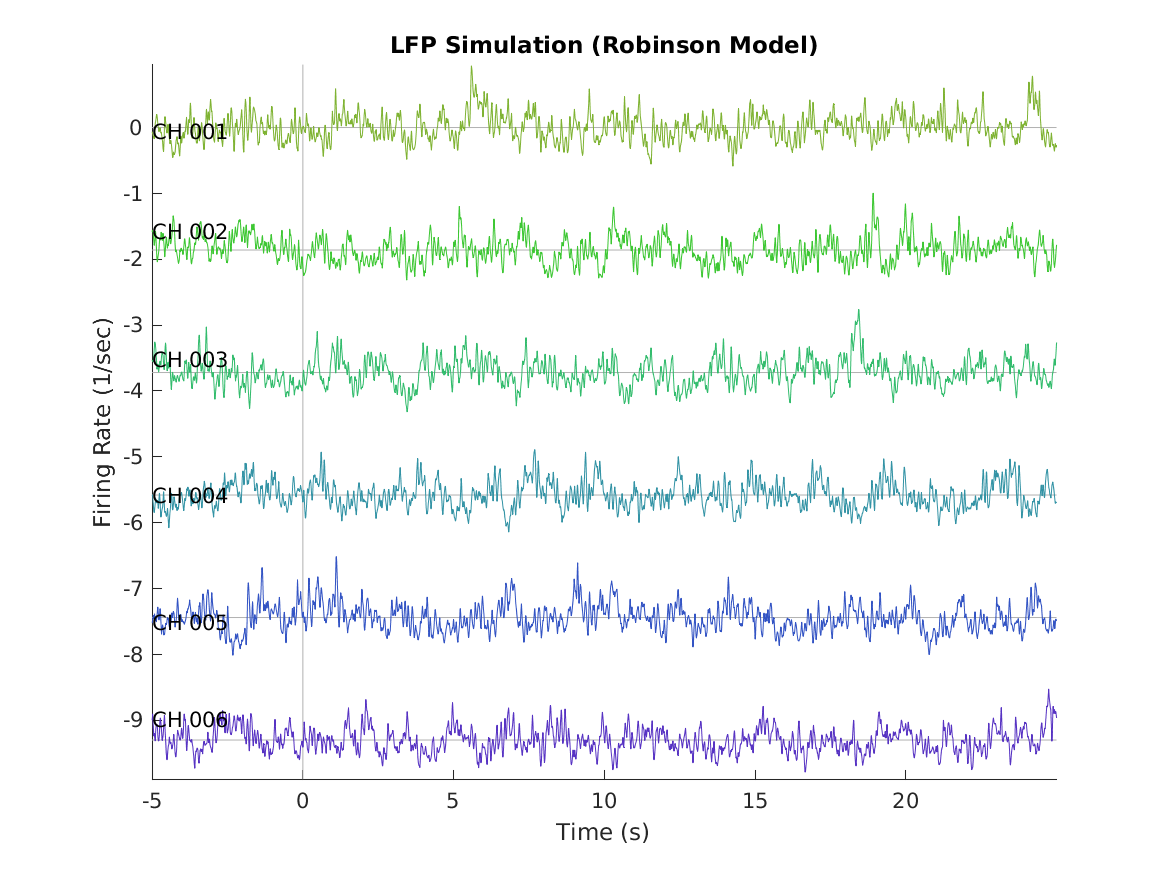
\includegraphics[width=5in]{plots/20231205/lfp-simulation-robinson-model}
%
\end{center}
%
\vfill
{\tiny \input{../LICENSE.md}}
%
\clearpage
%
%
% Front matter.
%
\pagestyle{plain}
\pagenumbering{roman}
\setcounter{page}{1}
%
\tableofcontents
%
\clearpage
%
%
% Document parts.
%
\pagestyle{plain}
\setcounter{page}{1}
\pagenumbering{arabic}
%
% Neuroloop utilities - Synthesis model guide - Overview
% Written by Christopher Thomas.

\chapter{Overview}
\label{sect-over}

This document describes the models used for synthesizing proxy neural
activity using the ``\texttt{nlSynth\_}'' family of library functions.

These functions are primarily intended to produce realistic-looking signals
with known qualities to test analysis scripts with. That said, these models
are drawn from publications where they were used to provide insight into
the functioning of brain networks, so using these functions for such
research is an additional use-case.

Chapter \ref{sect-robinson} describes the neural model presented in
Robinson 2002 (and elaborated on in Freyer 2011 and Hindriks 2023). This
is a model of average firing rates of multiple neural populations in the
cortex and thalamus, with feedback connections that drive noise-excited
oscillations.

\fixme{Other models go here once they're added.}

%
% This is the end of the file.

% Neuroloop utilities - Synthesis model guide - Robinson model
% Written by Christopher Thomas.

\chapter{Robinson Model}
\label{sect-robinson}

The model presented in Robinson 2002 (hereafter ``the Robinson model'')
provides a series of differential equations relating the firing rates of
multiple neural populations in the cortex and thalamus. Feedback between
these regions drives noise-excited oscillations.

The most relevant references are:
\begin{itemize}
\item Robinson 2002 -- Describes the model, finds steady-state points, and
analyzes perturbations around those points to find oscillation modes.
\item Freyer 2011 -- Describes an extension to the model where noise is
modulated by the network's own output, providing a closer match to the
distribution of oscillation modes in biological data.
\item Hindriks 2023 -- Describes an extension to the model that adds multiple
independent copies of the Robinson and Freyer model, with coupling between
instances. This is used to model co-oscillation of different brain regions
in biological data.
\end{itemize}
(See Section \ref{sect-robinson-refs} for citations.)

%
%
\section{Model Description}
\label{sect-robinson-model}

A diagram of the Robinson model with the extensions from Freyer 2011 and
Hindriks 2023 is shown in Figure \ref{fig-robinson-diagram}. To distinguish
this from the Robinson 2002 model, this will be referred to as ``the
extended Robinson model''.

\figdef{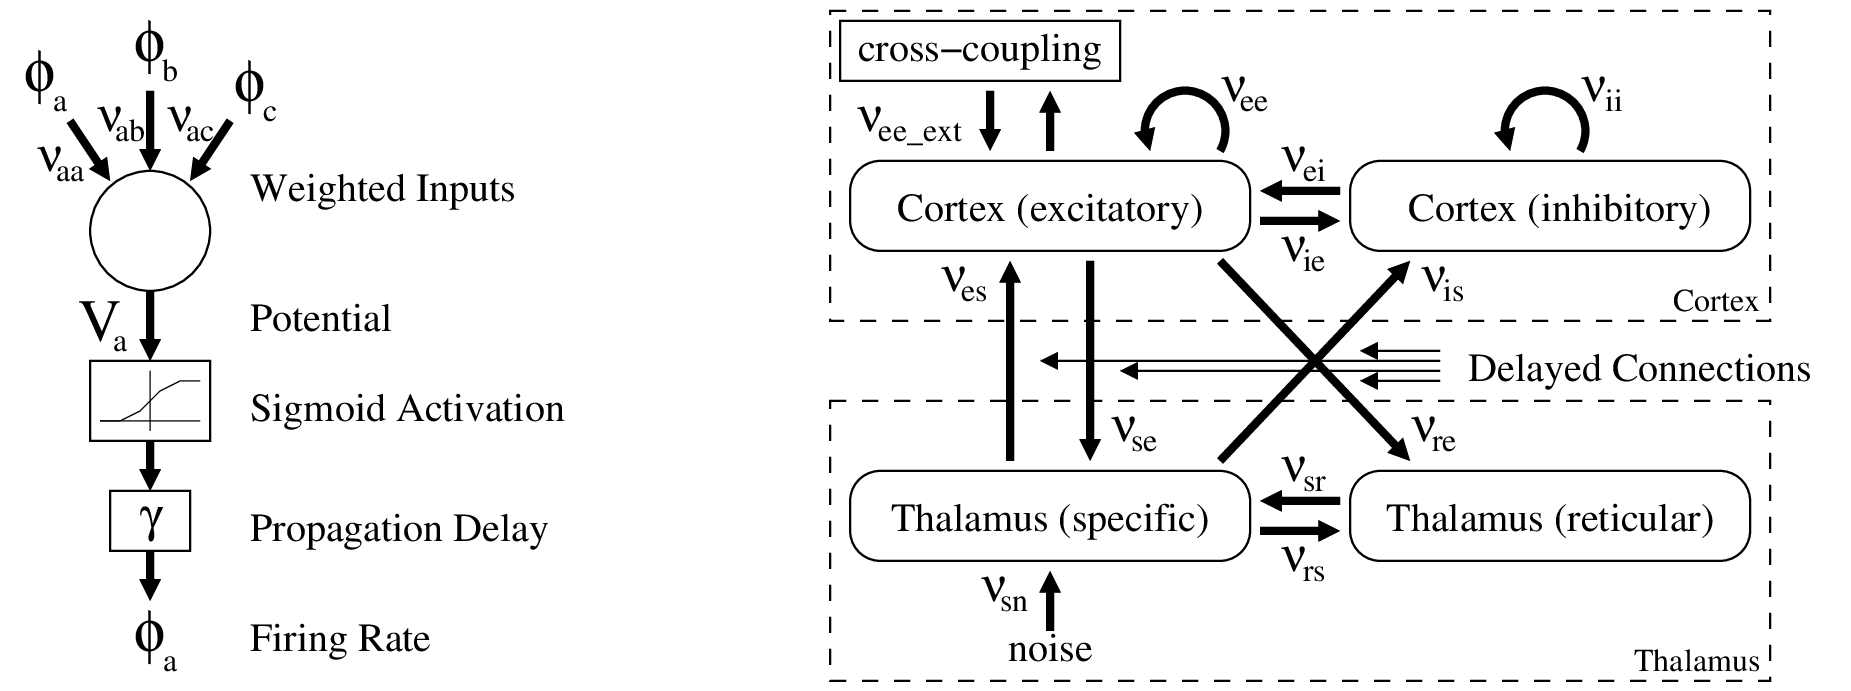
\includegraphics[width=0.9\columnwidth]{figures/robinson-model}}
{Extended Robinson model diagram, showing the neuron population model
(left) and the population interactions (right).}{fig-robinson-diagram}

The neural population model is described in Equations
\ref{eq-robinson-potential}, \ref{eq-robinson-sigmoid} and
\ref{eq-robinson-gamma}.
%
Per Equation \ref{eq-robinson-potential}, a weighted sum of input firing
rates $\phi_b(t)$ is used to generate the cell body potential $V_a(t)$. A
single dot indicates the first time derivative, and a double dot indicates
the second time derivative. The parameters $\alpha$ and $\beta$ are the
inverse of the membrane potential fall time and rise time, respectively.
The coupling parameter $\nu_{ab}$ is the strength of the connection from
region $b$ to region $a$ (zero if no connection, negative if inhibitory).

\textbf{NOTE:} A delay is manually applied to some of the $\phi_b$ signals
before this summation to reflect signal propagation time between the cortex
and thalamus (per Robinson 2002), and to reflect cross-coupling delays
within the cortex populations (per Hindriks 2023).

\begin{equation}
\left ( \frac{1}{\alpha \beta} \right ) \ddot{V}_a(t)
+ \left ( \frac{1}{\alpha} + \frac{1}{\beta} \right ) \dot{V}_a(t)
+ V_a(t) = \sum_b \nu_{ab} \phi_b(t)
\label{eq-robinson-potential}
\end{equation}

Per Equation \ref{eq-robinson-sigmoid}, the cell body potential $V$ is fed
into a sigmoid activation function, to represent the collective action of
many neurons with varying firing thresholds. The mean firing threshold is
$V_{th}$ and the standard deviation of the threshold is $\sigma_{th}$.
This follows the convention of Freyer 2011; Robinson 2002 defined a
related parameter $\sigma'_{th} = \frac{\sqrt{3}}{\pi} \sigma_{th}$ to
simplify the activation equation.

\begin{equation}
Q(V) = \frac{Q_{max}}
{1 + e^{- \left ( \frac{\pi}{\sqrt{3}} \right )
\left ( \frac{ V - V_{th}}{\sigma_{th}} \right )}}
\label{eq-robinson-sigmoid}
\end{equation}

Per Equation \ref{eq-robinson-gamma}, the local firing rate $Q$ is
propagated with damping and finite delay to give the non-local firing rate
$\phi$. A single dot indicates the first time derivative, and a double dot
indicates the second time derivative. Per Robinson 2002, local propagation
delay is assumed to only be relevant within the cortex, and
$\gamma = \infty$ is assumed elsewhere. Per Freyer 2011, this further only
applies to the excitatory neuron populations in the cortex.

\begin{equation}
\left \{
\begin{array}{rcl}
\frac{1}{\gamma^2} \ddot{\phi}(t) + \frac{2}{\gamma} \dot{\phi}(t) + \phi(t)
= Q(t) & ~~ & \mathrm{Cortex ~ excitatory ~ neurons.} \\
\phi(t) = Q(t) & ~~ & \mathrm{All ~ other ~ populations.} \\
\end{array}
\right .
\label{eq-robinson-gamma}
\end{equation}

Noise is injected into the model as $\phi_n$, and is described by Equation
\ref{eq-robinson-noise}. Per Freyer 2011, there are three components:
constant, additive, and multiplicative. Multiplicative noise (noise
modulated by $\phi_e$) is important for broadening the distribution of
peak power levels of transient oscillations at frequencies above the
fundamental oscillation mode of the cortex/thalamus loop.

In Equation \ref{eq-robinson-noise}, $\phi_n$ is the noise coupled to
the thalamus via $\nu_{sn}$, $\mu_n$ is the constant noise component
(background firing rate), $\sigma_n$ is the standard deviation of the
independent component of the noise, and $\chi$ is a scaling parameter
(per Freyer 2011) such that $\sigma_n \chi$ is the standard deviation of
the component of the noise that is modulated by $\phi_e$. Since the $\phi_e$
signal has to propagate from the cortex to the thalamus before modulating
this noise component, it is manually delayed. The signals $g_1(t)$ and
$g_2(t)$ denote two independent Gaussian noise sources with zero mean and
with standard deviations of 1.

\begin{equation}
\phi_n(t) = \mu_n + \sigma_n g_1(t)
+ \sigma_n \chi g_2(t) \phi_e(t - t_{halfloop})
\label{eq-robinson-noise}
\end{equation}

As shown in Figure \ref{fig-robinson-diagram}, cross-coupling between
excitatory cortical populations is implemented per Hindriks 2023. This is
described by Equation \ref{eq-robinson-coupling}. Weight values
$w_{ab}$ represent the strength of connections between populations, and
delay values $t_{coupling_{ab}}$ represent the propagation delays of these
connections.
While arbitrary weight values may be chosen, the recommended implementation
is to use positive weights (purely excitatory), with the constraint that the
sum of all weights contributing to a given $\phi_{ext_k}$ should sum to
approximately unity. Cross-coupling propagation delay is typically no more
than $\frac{1}{\gamma}$.

\begin{equation}
\phi_{ext_a}(t) = \sum_b w_{ab} \phi_e(t - t_{coupling_{ab}})
\label{eq-robinson-coupling}
\end{equation}

\begin{equation}
\forall a, \sum_b w_{ab} \approx 1
\label{eq-robinson-coupling-constraint}
\end{equation}

Typical parameter values for the extended Robinson model are shown in
Table \ref{tab-robinson-params}. Typical coupling coefficients are shown in
Table \ref{tab-robinson-couplings}. These are very similar to the parameter
and coupling coefficient values used in Hindriks 2023.

\tabdef{%
\begin{tabular}{cccl}\hline
\textbf{Parameter} & \textbf{Value} & \textbf{Units} & \textbf{Notes} \\
\hline
$Q_{max}$ & 250 & sec$^{-1}$ & maximum firing rate \\
$V_{th}$ & 15 & mV & potential threshold for firing \\
$\sigma_{th}$ & 6 & mV & standard deviation of firing threshold \\
\hline
$\alpha$ & 50 & sec$^{-1}$ & membrane potential inverse fall time \\
$\beta$ & 200 & sec$^{-1}$ & membrane potential inverse rise time \\
$\gamma$ & 100 & sec$^{-1}$ & cortex inverse propagation delay \\
\hline
$t_{halfloop}$ & 40 & ms & one-way cortex/thalamus delay \\
\hline
$\mu_n$ & 0 & sec$^{-1}$ & constant noise firing rate \\
$\sigma_n$ & 0.1 & sec$^{-1}$ & additive noise standard deviation \\
$\chi$ & 0.3 & dimensionless & multiplicative noise deviation coefficient \\
\hline
\end{tabular}
}{Typical parameters for the extended Robinson model.}
{tab-robinson-params}

\tabdef{%
\begin{tabular}{cc}
\hline
$\nu_{ee}$ & 1.2 \\
$\nu_{ei}$ & -1.8 \\
$\nu_{es}$ & 1.2 \\
\hline
$\nu_{ie}$ & 1.2 \\
$\nu_{ii}$ & -1.8 \\
$\nu_{is}$ & 1.2 \\
\hline
$\nu_{se}$ & 1.2 \\
$\nu_{re}$ & 0.4 \\
\hline
$\nu_{sr}$ & -0.8 \\
$\nu_{rs}$ & 0.2 \\
\hline
$\nu_{sn}$ & 0.5 \\
\hline
$\nu_{ee_{ext}}$ & 0.07 \\
\hline
\end{tabular}
}{Typical coupling coefficient values for the extended Robinson model.}
{tab-robinson-couplings}
%
% FIXME - Flush floats.
\clearpage

%
%
\section{Discussion}
\label{sect-robinson-discussion}

Applying the Laplace transform to Equation \ref{eq-robinson-potential} shows
that the effect of $\alpha$ and $\beta$ is to apply a low-pass filter to the
weighted sum of input firing rates (a second-order exponential smoothing
filter with poles at $-\alpha$ and $-\beta$).

\begin{equation}
\left ( \frac{1}{\alpha \beta} \right ) s^2 V_a(s)
+ \left ( \frac{1}{\alpha} + \frac{1}{\beta} \right ) s V_a(s)
+ V_a(s) = \sum_b \nu_{ab} \Phi_b(s)
\end{equation}
%
\begin{equation}
s^2 V_a(s) + (\alpha + \beta) s V_a(s) + \alpha \beta V_a(s)
= \alpha \beta \sum_b \nu_{ab} \Phi_b(s)
\end{equation}
%
\begin{equation}
(s + \alpha) (s + \beta) V_a(s) = \alpha \beta \sum_b \nu_{ab} \Phi_b(s)
\end{equation}
%
\begin{equation}
\frac{V_a(s)}{\sum_b \nu_{ab} \Phi_b(s)}
= \frac{\alpha \beta}{(s + \alpha) (s + \beta)}
\end{equation}

Applying the Laplace transform to Equation \ref{eq-robinson-gamma} shows
that the effect of $\gamma$ is to apply a low-pass filter to the firing rate
(a second-order exponential smoothing filter with both poles at $-\gamma$).

\begin{equation}
\left ( \frac{1}{\gamma^2} \right ) s^2 \Phi(s)
+ \left ( \frac{2}{\gamma} \right ) s \Phi(s) + \Phi(s) = Q(s)
\end{equation}
%
\begin{equation}
s^2 \Phi(s) + 2 \gamma s \Phi(s) + \gamma^2 \Phi(s) = \gamma^2 Q(s)
\end{equation}
%
\begin{equation}
(s + \gamma)^2 \Phi(s) = \gamma^2 Q(s)
\end{equation}
%
\begin{equation}
\frac{\Phi(s)}{Q(s)} = \frac{\gamma^2}{(s + \gamma)^2}
\end{equation}

The fundamental-mode oscillation is usually supported by resonance in the
cortico-thalamic loop, with a period near $2 \cdot t_{halfloop}$ (alpha band
for $t_{halfloop}$ of 40~ms). The first overtone mode can support beta band
oscillations. If coupling values are chosen such that the system is only
barely stable near these resonance modes, oscillatory bursts can occur.

Robinson 2002 gives a detailed description of how this stability analysis
may be performed. For some regions of parameter space, multiple operating
points exist. With parameter values chosen from these regions, the system
will switch between several states with different oscillation
characteristics. The parameter values used in Freyer 2011 and Hindriks 2023
were chosen to exploit this behavior.

%
%
\section{References}
\label{sect-robinson-refs}

\begin{itemize}
%
\item P. A. Robinson, C. J. Rennie, and D. L. Rowe, \textit{Dynamics of
Large-Scale Brain Activity in Normal Arousal States and Epileptic Seizures},
Physical Review E, 65, 041924, April 2002
%
\item F. Freyer, J. A. Roberts, R. Becker, P. A. Robinson, P. Ritter, and
M. Breakspear, \textit{Biophysical Mechanisms of Multistability in
Resting-State Cortical Rhythms}, Journal of Neuroscience, 31,
pp 6353--6361, April 2011
%
\item R. Hindriks and P. K. B. Tewarie, \textit{Dissociation Between Phase
and Power Correlation Networks in the Human Brain is Driven by Co-Occurrent
Bursts}, Communications Biology, 6, 286, March 2023
%
\end{itemize}

%
%
% This is the end of the file.

% Neuroloop utilities - Synthesis model guide - Robinson model - Analysis
% Written by Christopher Thomas.

\section{Mathematical Analysis}
\label{sect-robinson-math}

%
%
\subsection{Low-Pass Filter Delays}
\label{sect-robinson-math-lowpass}

Applying the Laplace transform to Equation \ref{eq-robinson-potential} shows
that the effect of $\alpha$ and $\beta$ is to apply a low-pass filter to the
weighted sum of input firing rates (a second-order exponential smoothing
filter with poles at $-\alpha$ and $-\beta$).

\begin{equation}
\left ( \frac{1}{\alpha \beta} \right ) s^2 V_a(s)
+ \left ( \frac{1}{\alpha} + \frac{1}{\beta} \right ) s V_a(s)
+ V_a(s) = \sum_b \nu_{ab} \Phi_b(s)
\end{equation}
%
\begin{equation}
s^2 V_a(s) + (\alpha + \beta) s V_a(s) + \alpha \beta V_a(s)
= \alpha \beta \sum_b \nu_{ab} \Phi_b(s)
\end{equation}
%
\begin{equation}
(s + \alpha) (s + \beta) V_a(s) = \alpha \beta \sum_b \nu_{ab} \Phi_b(s)
\end{equation}
%
\begin{equation}
\frac{V_a(s)}{\sum_b \nu_{ab} \Phi_b(s)}
= \frac{\alpha \beta}{(s + \alpha) (s + \beta)}
\end{equation}

Applying the Laplace transform to Equation \ref{eq-robinson-gamma} shows
that the effect of $\gamma$ is to apply a low-pass filter to the firing rate
(a second-order exponential smoothing filter with both poles at $-\gamma$).

\begin{equation}
\left ( \frac{1}{\gamma^2} \right ) s^2 \Phi(s)
+ \left ( \frac{2}{\gamma} \right ) s \Phi(s) + \Phi(s) = Q(s)
\end{equation}
%
\begin{equation}
s^2 \Phi(s) + 2 \gamma s \Phi(s) + \gamma^2 \Phi(s) = \gamma^2 Q(s)
\end{equation}
%
\begin{equation}
(s + \gamma)^2 \Phi(s) = \gamma^2 Q(s)
\end{equation}
%
\begin{equation}
\frac{\Phi(s)}{Q(s)} = \frac{\gamma^2}{(s + \gamma)^2}
\end{equation}

The effect of both of these filters is to suppress high-frequency
oscillations (those above the filter corner frequencies) and to delay
low-frequency oscillations by an amount approximately equal to the filters'
time constants. These delays and corner frequencies are listed in Table
\ref{tab-robinson-lowpass} (using the parameter values from
\ref{tab-robinson-params}).

\tabdef{%
\begin{tabular}{cccc}\hline
\textbf{Parameter} & \textbf{Value} & \textbf{Corner} & \textbf{Delay} \\
\hline
$\alpha$ & 50 sec$^{-1}$ & 8 Hz & 20 ms \\
$\beta$ & 200 sec$^{-1}$ & 32 Hz & 5 ms \\
$\gamma$ & 100 sec$^{-1}$ & 16 Hz & 20 ms$^*$ \\
\hline
\multicolumn{4}{l}
{\footnotesize $^*$Each pole at $-\gamma$ introduces a 10~ms delay; there
are two such poles.}
\end{tabular}
}{Robinson model low-pass filter corners and low-frequency delays.}
{tab-robinson-lowpass}

%
%
\subsection{Oscillation Modes}
\label{sect-robinson-math-modes}

A simplified diagram of the extended Robinson model is shown in Figure
\ref{fig-robinson-loops}. This is intended to make it easy to identify the
feedback loops that may support oscillations. Blue arcs indicate positive
coefficients, and red arcs indicate negative (inhibitory) coefficients.
As an approximation, the activity of different excitatory neuron populations
within the cortex is assumed to be the same, combining $\nu_{ee}$ and
$\nu_{ee\_ext}$. Additionally, multiplicative portion of the noise is
treated as a contribution to the $\nu_{se}$ arc. The average contribution of
the $\chi \sigma_n \nu_n$ term is zero, but the magnitude of that term
compared to the magnitude of $\nu_{se}$ indicates whether or not
multiplicative noise significantly contributes to that arc.

\figdef{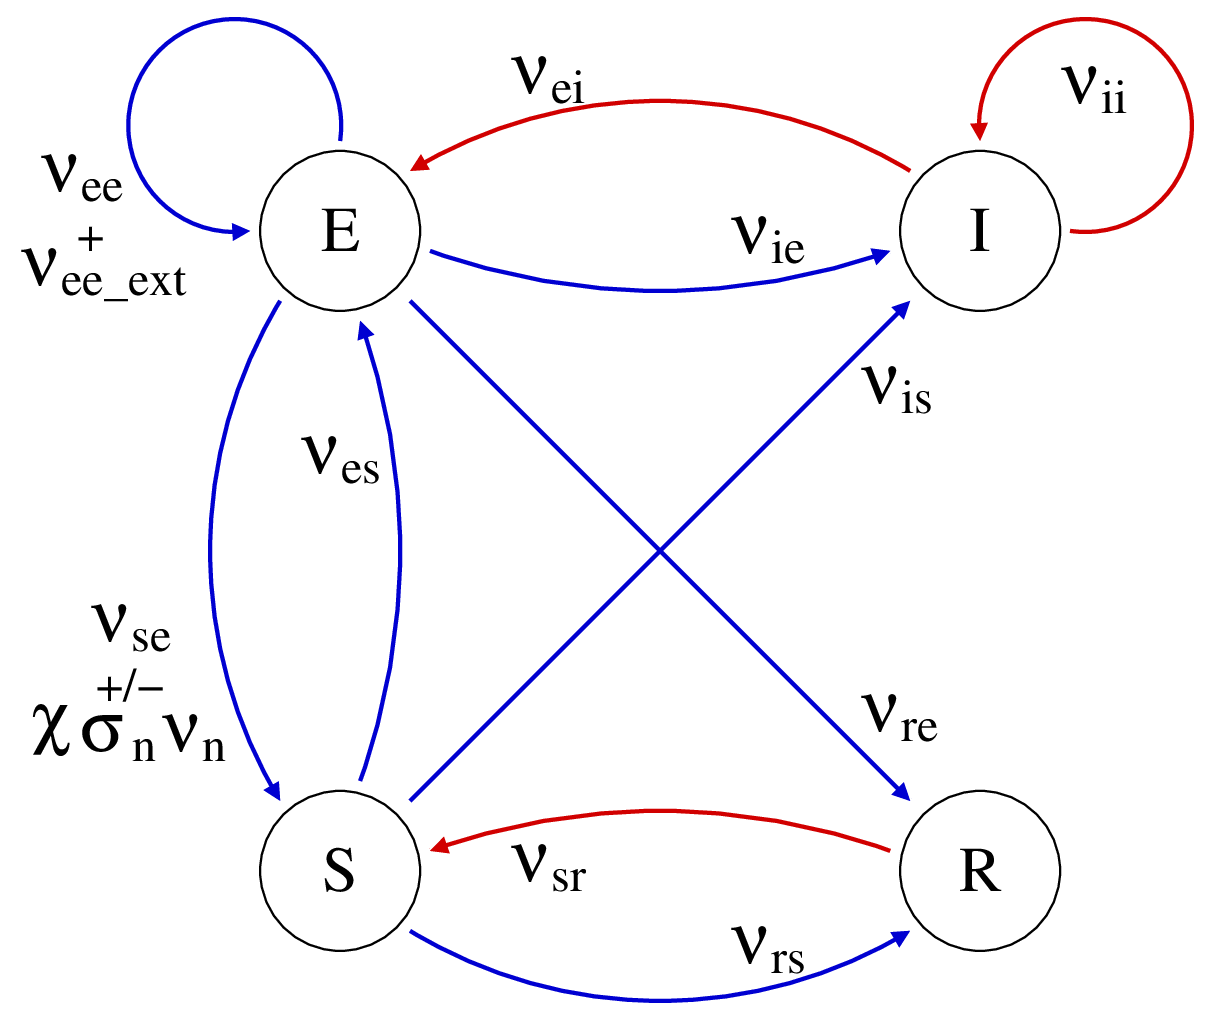
\includegraphics[height=2.5in]{figures/robinson-model-loops}}
{Simplified diagram of the extended Robinson model, showing feedback loops.}
{fig-robinson-loops}

A list of potential oscillation loops and their oscillation frequencies is
given in Table \ref{tab-robinson-loops}. For loops consisting entirely of
positive coefficients, the oscillation period is the time needed to complete
a single circuit. For loops with one negative coefficient, the oscillation
period is the time needed to complete two circuits around the loop (in the
same manner as a ring oscillator). Harmonics of these oscillation frequencies
are also supported.

The number of arc traversals needed for one oscillation period is noted.
Per above, this may reflect either one or two cycles around the loop. Each
arc traversal involves gain from arc coefficients (noted in the table),
small-signal gain from the $Q(V)$ transfer function (omitted from the table),
and delay from the $\alpha$ and $\beta$ filter components. Delay
contributions from the cortex excitatory population $\gamma$ filter
component and from the cortex-thalamus loop are noted in the table where
applicable.

\tabdef{%
\begin{tabular}{ccccccc}\hline
\textbf{Label} & \textbf{Arcs} & \textbf{Gamma} & \textbf{C-T Loop} &
\textbf{Period} & \textbf{Frequency} & \textbf{Gain} \\
\hline
ES & 2 & Y & Y & 150 ms & 6.7 Hz & $\nu_{se} \cdot \nu_{es}$ \\
EE & 1 & Y & -- & 45 ms & 22 Hz & $\nu_{ee} + \nu_{ee\_ext}$ \\
\hline
EI & 4 & Y & -- & 140 ms & 7 Hz & $2 \cdot \nu_{ie} \cdot \nu_{ei}$ \\
SR & 4 & -- & -- & 100 ms & 10 Hz & $2 \cdot \nu_{rs} \cdot \nu_{sr}$ \\
%
ERS & 6 & Y & Y & 350 ms & 2.9 Hz &
$2 \cdot \nu_{re} \cdot \nu_{sr} \cdot \nu_{es}$ \\
ESI & 6 & Y & Y & 350 ms & 2.9 Hz &
$2 \cdot \nu_{se} \cdot \nu_{is} \cdot \nu_{ei}$ \\
\hline
\end{tabular}
}{Extended robinson model oscillation modes. Top two modes: single-cycle.
Bottom four modes: two-cycle (inverting). Activation function gain is
not shown.}
{tab-robinson-loops}

Resonant loops explicitly described in Section IV of Robinson 2002 are the
ones marked ES, ERS, and SR. The oscillation periods described in Section
V of Robinson 2002 are consistent with the estimated periods of the ERS and
SR loops in Table \ref{tab-robinson-loops}.

The authors of Robinson 2002 were primarily concerned with noise-excited
oscillations, and so only evaluated oscillation loops that included the
specific nucleus. Evaluation was expressed in terms of the transfer
function from the noise signal (input) to the firing rate of cortex
excitatory neurons (output). Resonant oscillations were presumed to occur
at frequencies for which this transfer function diverged (producing
arbitrarily large output for finite input). This work instead considers
gain within a loop, with resonant oscillations corresponding to a loop
gain exceeding unity. As this does not explicitly consider noise excitation,
all of the loops described in Table \ref{tab-robinson-loops} may be
analyzed.

\subsection{Operating Points}
\label{sect-robinson-math-fixed}

As was described in Robinson 2002, the dynamics of the extended Robinson
model can be analyzed by considering unchanging (DC) firing rates, and
evaluating the small-signal gain around these operating points. While this
was used to find the transfer function
$\frac{\phi_e(\omega)}{\phi_n(\omega)}$ in Robinson 2002, here it is used
to find the small-signal loop gain (to determine which oscillating modes
are dominant for given parameter values).

At a given operating point, the sensitivity of the gain of the dominant
loops to each of the $v_{ab}$ coefficients provides insight into which
network connections are most relevant for influencing dynamcis at that
operating point. $v_{ee\_ext}$ is particularly of interest, as this
may be used as a proxy for the sensitivity of network dynamics to changes
in the connectivity matrix between different excitatory cortex neuron
populations.

For time-independent operating point analysis, Equation
\ref{eq-robinson-potential} reduces to:

\begin{equation}
V_a = \sum_b \nu_{ab} \phi_b
\label{eq-robinson-dc-potential}
\end{equation}

Equation \ref{eq-robinson-sigmoid} (defining $Q(V)$) is unchanged, and
Equation \ref{eq-robinson-gamma} reduces to:

\begin{equation}
\phi_a = Q(V_a)
\label{eq-robinson-dc-nogamma}
\end{equation}

Combining Equations \ref{eq-robinson-dc-potential} and
\ref{eq-robinson-dc-nogamma} gives:

\begin{equation}
V_a = \sum_b \nu_{ab} Q(V_b)
\label{eq-robinson-dc-scalar}
\end{equation}
%
\begin{equation}
\vec{V} = \mathbf{N} Q(\vec{V})
\label{eq-robinson-dc-vector}
\end{equation}

In Equation \ref{eq-robinson-dc-vector}, vector $\vec{V}$ contains as its
elements all $V_a$, matrix $\mathbf{N}$ contains as its elements all
$\nu_{ab}$, and the activation function Q acts separately on each element
of $\vec{V}$.

The activation function given in \ref{eq-robinson-sigmoid-prime} can be
rewritten as:

\begin{equation}
Q(V) = \frac{Q_{max}}{1 +
e^{\left ( \frac{V_{th}}{\sigma'_{th}} \right )}
e^{- \left ( \frac{V}{\sigma'_{th}} \right )}
}
\label{eq-robinson-sigmoid-shuffle-1}
\end{equation}

For firing rates that are much less than $Q_{max}$ (such as those plotted
in Robinson 2002), the exponential term dominates, and the activation
function can be approximated as:

\begin{equation}
Q(V) \approx Q_{max} \, e^{- \left ( \frac{V_{th}}{\sigma'_{th}} \right )}
e^{\left ( \frac{V}{\sigma'_{th}} \right )}
\label{eq-robinson-sigmoid-approx-full}
\end{equation}
%
\begin{equation}
Q(V) \approx Q_0 \, e^{\left ( \frac{V}{\sigma'_{th}} \right )}
\label{eq-robinson-sigmoid-approx}
\end{equation}
%
\begin{equation}
Q_0 = Q_{max} \, e^{- \left ( \frac{V_{th}}{\sigma'_{th}} \right )}
\label{eq-robinson-sigmoid-q0}
\end{equation}

The operating point equation then becomes Equation
\ref{eq-robinson-dc-vector-approx}, where exponentiation is performed
separately for each element of $\vec{V}$:

\begin{equation}
\vec{V} \approx
\mathbf{N} \, Q_0 \, e^{\left ( \frac{\vec{V}}{\sigma'_{th}} \right )}
\label{eq-robinson-dc-vector-approx}
\end{equation}

While this system of equations may be solved numerically (and was solved
numerically in Robinson 2002), an estimate of the operating point may be
obtained by assuming that potentials are small compared to $\sigma'_{th}$.
\textbf{This is not a robust assumption;} it is used as an estimate only.
With this caveat kept in mind, a linear approximation of the exponential
function may be used (the first-order Taylor expansion), giving the following
(where $\vec{1}$ denotes a vector where all elements are unity):

\begin{equation}
\vec{V} \approx \mathbf{N} \, Q_0 \,
\left [ \vec{1} + \left ( \frac{1}{\sigma'_{th}} \right ) \vec{V} \right ]
\end{equation}
%
\begin{equation}
\left ( \frac{1}{Q_0} \right ) \vec{V} \approx \mathbf{N} \, \vec{1}
+ \left ( \frac{1}{\sigma'_{th}} \right ) \mathbf{N} \, \vec{V}
\end{equation}
%
\begin{equation}
\left [ \left ( \frac{1}{Q_0} \right ) \mathbf{I}
- \left ( \frac{1}{\sigma'_{th}} \right ) \mathbf{N}
\right ] \vec{V} \approx \mathbf{N} \, \vec{1}
\label{eq-robinson-dc-vector-linear}
\end{equation}

Equation \ref{eq-robinson-dc-vector-linear} has the form
$\mathbf{A} \vec{V} = \vec{b}$, and so may be solved as a set of linear
equations. The operating point estimated using Equation
\ref{eq-robinson-dc-vector-linear} \textbf{must} be examined to confirm
that $|V_a| \ll \sigma'_{th}$ for all $V_a$. If this constraint does not
hold, the estimate is not correct.

%
%
\subsection{Small-Signal Gain and Dominant Oscillations}
\label{sect-robinson-math-gain}

The small-signal gain $G_{ab}$ of any given arc is the derivative of its
output firing rate with respect to its input firing rate. For oscillations
with frequencies much lower than the $\alpha$, $\beta$, and $\gamma$ filter
corner frequencies, this may be estimated by taking the derivative of the
DC operating point equations (rather than requiring an analysis of the full
system dynamics):

\begin{equation}
G_{ab} = \frac{d\phi_a}{d\phi_b}
\approx \frac{d}{d\phi_b} \left [ Q(V_a) \right ]
\end{equation}
%
\begin{equation}
G_{ab} \approx Q'(V_a) \frac{dV_a}{d\phi_b}
\end{equation}
%
\begin{equation}
G_{ab} \approx
Q'(V_a) \frac{d}{d\phi_b} \left [ \sum_c \nu_{ac} \phi_c \right ]
\end{equation}
%
\begin{equation}
G_{ab} \approx Q'(V_a) \nu_{ab}
\label{eq-robinson-gain-qprime}
\end{equation}

The sigmoid response function is defined in terms of the logistic function:

\begin{equation}
\left \{
\begin{array}{l}
Q(V) = Q_{max} L \left (\frac{V - V_{th}}{\sigma'_{th}} \right ) \\
\\
L(x) = \frac{1}{1 + e^{-x}} = \frac{e^x}{1 + e^x} \\
\\
\sigma'_{th} = \frac{\sqrt{3}}{\pi}\sigma_{th} \\
\end{array}
\right .
\label{eq-robinson-sigmoid-logistic}
\end{equation}

The derivative of the logistic function is:

\begin{equation}
L'(x) = L(x) \left ( 1 - L(x) \right ) = \frac{e^x}{(1 + e^x)^2}
\label{eq-robinson-logistic-derivative}
\end{equation}

This gives the derivative of the sigmoid response function:

\begin{equation}
Q'(V) = Q_{max} L' \left ( \frac{V - V_{th}}{\sigma'_{th}} \right )
\frac{d}{dV} \left [ \frac{V - V_{th}}{\sigma'_{th}} \right ]
\end{equation}
%
\begin{equation}
Q'(V) = \frac{Q_{max}}{\sigma'_{th}}
L' \left ( \frac{V - V_{th}}{\sigma'_{th}} \right )
\end{equation}
%
\begin{equation}
Q'(V) = \frac{Q_{max}}{\sigma'_{th}}
L \left ( \frac{V - V_{th}}{\sigma'_{th}} \right )
\left ( 1 - L \left ( \frac{V - V_{th}}{\sigma'_{th}} \right ) \right )
\end{equation}
%
\begin{equation}
Q'(V) = \frac{Q_{max}}{\sigma'_{th}}
L \left ( \frac{V - V_{th}}{\sigma'_{th}} \right )
\left ( 1 - \frac{Q_{max}}{Q_{max}}
L \left ( \frac{V - V_{th}}{\sigma'_{th}} \right ) \right )
\end{equation}
%
\begin{equation}
Q'(V) = \frac{1}{\sigma'_{th}} Q(V) \left ( 1 - \frac{Q(V)}{Q_{max}} \right )
\end{equation}

Combining this with Equation \ref{eq-robinson-gain-qprime} gives:

\begin{equation}
G_{ab} \approx \frac{\nu_{ab}}{\sigma'_{th}}
Q(V_a) \left ( 1 - \frac{Q(V_a)}{Q_{max}} \right )
\end{equation}
%
\begin{equation}
G_{ab} \approx \frac{\nu_{ab}}{\sigma'_{th}}
\phi_a \left ( 1 - \frac{\phi_a}{Q_{max}} \right )
\label{eq-robinson-gain}
\end{equation}

This is Equation 10 from Robinson 2002. The small-signal gain of a loop at
low frequencies is the product of $G_{ab}$ for each arc in the loop
(as with the $S_d$, $S_i$, and $S_r$ values in section IV of Robinson 2002).


\fixme{Add code for using the model to generate rates.}

\fixme{Add code for finding operating points, both as estimates and via
brute force numerical solutions.}

\fixme{Show how to evaluate loop gain and envelope time constants.}

\fixme{Show how to find regions of parameter space where desired loops are
dominant, including ones where the mixing matrix matters. Show where the
regions Robinson plotted are. Show where the region Hindriks used is.}

%
%
% This is the end of the file.

%
%
\end{document}

%
% This is the end of the file.
